%%%%%%%%%%%%%%%%%%%%%%%%%%%%%%%%%%%%%%%%%%
%%% NORMALMENTE NO ES NECESARIO HACER 
%%% CAMBIOS EN ESTA PARTE DEL DOCUMENTO
%%%%%%%%%%%%%%%%%%%%%%%%%%%%%%%%%%%%%%%%%%


%:Clase del documento
\documentclass[fontsize=11pt, Myfinal=true, twoside, numbers=noenddot]{scrbook}
%Minion=true, English=true, Myfinal=true

%:Paquete de estilos propuesto
\usepackage{libroETSI}

%:Paquete específico para cargar tikz (y sus librerías) y pgfplots
\usepackage{dtsc-creafig}

%:Paquete para notaciones específicas
\usepackage{notacion}

%:Paquete para incorporar aspectos concretos de la edición
\usepackage{edicionPFC}

% Paquete para incluir epígrafes en los capítulos
\usepackage{epigraph}

% Paquete para incluir glosario
\usepackage{glossaries}

%:Para modificar fácilmente la fuente del texto.
\makeatletter
\ifdtsc@Minion % Queremos utilizar la fuente Minion y lo hemos declarado al principio
	\ifluatex
		\setmainfont[Renderer=Basic, Ligatures=TeX,	% Fuente del texto 
		Scale=1.01,
		]{Minion Pro}
   		% En este caso conviene modificar ligeramente el tamaño de las fuentes matemáticas
		\DeclareMathSizes{10}{10.5}{7.35}{5.25}
		\DeclareMathSizes{10.95}{11.55}{8.08}{5.77}
		\DeclareMathSizes{12}{12.6}{8.82}{6.3}
%		\setmainfont[Renderer=Basic, Ligatures=TeX,	% Fuente del texto 
%		]{Adobe Garamond Pro}
%		\setmainfont[Renderer=Basic, Ligatures=TeX,	% Fuente del texto 
%		]{Palatino LT Std}
	\fi
\else
	\ifluatex
		% Para utilizar la fuente Times New Roman, o alguna otra que se tenga instalada
		\setmainfont[Renderer=Basic, Ligatures=TeX,	% Fuente del texto 
		Scale=1.0,
		]{Times New Roman}
	\else
		\usepackage{tgtermes} 	%clone of Times
		%\usepackage[default]{droidserif}
		%\usepackage{anttor} 	
	\fi
\fi
\makeatother

% Formato A4
\geometry
{paperheight=297mm,%
paperwidth=210mm,%
top=25mm,%
headsep=8.5mm,%
includefoot, 
textheight=240mm, 
textwidth=150mm, 
bindingoffset=0mm, 
twoside}

\usepackage[a4,center]{crop}%para poner las cruces de esquina de página, poner la opción cross

%:Esquema de numeración por defecto
\setenumerate[1]{label=\normalfont\bfseries{\arabic*.}, leftmargin=*, labelindent=\parindent}
\setenumerate[2]{label=\normalfont\bfseries{\alph*}), leftmargin=*}
\setenumerate[3]{label=\normalfont\bfseries{\roman*.}, leftmargin=*}
\setlist{itemsep=.1em}
\setlength{\parindent}{1.0 em}

\setcounter{tocdepth}{4}						% El nivel hasta el que se muestra el índice 


%%%%%%%%%%%%%%%%%%%%%%%%%%%%%%%%%%%%%%%%%%
%%% A PARTIR DE AQUÍ HAY QUE EDITAR
%%%%%%%%%%%%%%%%%%%%%%%%%%%%%%%%%%%%%%%%%%

% Ejemplo de Glosario
\newacronym[type=main]{ETSI}{ETSI}{Escuela Técnica Superior de Ingeniería}
\newacronym[type=main]{US}{US}{Universidad de Sevilla}
\newacronym[type=main]{SEU}{SEU}{Single Event Upset}
\newacronym[type=main]{SEE}{SEE}{Single Event Effect}
\newacronym[type=main]{TMR}{TMR}{Triple Modular Redundancy}
\newacronym[type=main]{RBM}{RBM}{Restricted Boltzmann Machine}
\newacronym[type=main]{CUT}{CUT}{Circuit Under Test}
\newacronym[type=main]{FF}{FF}{flip-flop}
\newacronym[type=main]{ESA}{ESA}{European Space Agency}
\newacronym[type=main]{FPGA}{FPGA}{Field Programmable Gate Array}
%\newacronym[type=main]{}{}{}


\makeindex
\makeglossaries %Si no se quiere el glosario, comentar esta línea.


%:Empieza el documento

\begin{document}


%PORTADA
%ver edicionPFC.sty para modificaciones

%:Para crear la portada y la portada interior (pagina titular)
\titulo{Técnica de diagnóstico de SEU utilizando diccionarios de fallos incompletos} %\mbox evita que se divida una palabra al cambiar de línea
\autor{Álvaro Calvo Matos}
\director{Hipólito Guzmán Miranda}
\titulodirector{Profesor Titular}

\departamento{Dpto. Ingeniería Electrónica}
\centro{Escuela Técnica Superior de Ingeniería}
\universidad{Universidad de Sevilla}
\titulacion{Grado en Ingeniería Electrónica, Robótica y \mbox{Mecatrónica}}
\fecha{2020}
\nombretrabajo{Trabajo Fin de Grado} %Proyecto fin de Máster,....

\hypersetup
	{
 	linkcolor=black, %Tocar para poner color en enlaces
	pdfauthor={\elautor},
	pdftitle={\nombretrabajo,\eltitulo}, 
	pdfkeywords={Latex, edición, formato de texto}	
	 }

\portadaPFC{figuras/LogoUS.pdf}{figuras/LogoTSC.pdf} %logo de la Universidad y logo del departamento, si lo hubiera. Para cambiar el pie de página con los logos, debe editarse el fichero ediciónPFC.sty

%%%%%%%%%%%%%%%%%%%%%%%%%%%%%%%%%%%%%%%%%%%%%%%%%%%%%%%%%%%%%%%%%%%%%%%%%%%%%%%%
% Para incluir el logo del departamento hay que modificar el segundo parámetro entregado en la linea 127 de este .tex, y
% hay que modificar las lineas 92 a 100 del fichero "edicionPFC.sty"

%Fin Portada

%:Todo lo que constituye la primera parte del libro que no es el cuerpo del libro en realidad
\frontmatter
\pagenumbering{Roman} %Pone la numeración en mayúscula (En español parece que es obligatorio)

%\include{dedicatoria/dedicatoria}%¿Comentar para proyectos/tesis?
% !TEX root =../LibroTipoETSI.tex
\chapter*{Agradecimientos}
%\pagestyle{especial}
\pagestyle{empty}
%\chaptermark{Agradecimientos}
\phantomsection
%\addcontentsline{toc}{listasf}{Agradecimientos}
%\vspace{1cm}
%{\huge{Agradecimientos}}
%\vspace{1cm}

\lettrine[lraise=-0.1, lines=2, loversize=0.25]{E}{l} diseño de una hoja de estilo en \LaTeX\ para un texto no es en absoluto trivial. Por un lado hay que conocer bien los usos, costumbres y reglas que se emplean a la hora de establecer márgenes, tipos de letras, tamaños de las mismas, títulos, estilos de tablas, y un sinfín de otros aspectos. Por otro, la programación en \LaTeX\ de esta hoja de estilo es muy tediosa, incluida la selección de los mejores paquetes para ello. La hoja de estilo adoptada por nuestra Escuela y utilizada en este texto es una versión de la que el profesor Payán realizó para un libro que desde hace tiempo viene escribiendo para su asignatura. Además, el prof. Payán ha participado de forma decisiva en la adaptación de dicha plantilla a los tres tipos de documentos que se han tenido en cuenta: libro, tesis y proyectos final de carrera, grado o máster. Y también en la redacción de este texto, que sirve de manual para la utilización de estos estilos. Por todo ello, y por hacerlo de forma totalmente desinteresada, la Escuela le está enormemente agradecida.

A esta hoja de estilos se le incluyó unos nuevos diseños de portada. El diseño gráfico de las portadas para proyectos fin de grado, carrera y máster, está basado en el que el prof. Fernando García García, de la Facultad de Bellas Artes de nuestra Universidad, hiciera para los libros, o tesis, de la sección de publicación de nuestra Escuela. Nuestra Escuela le agradece que pusiera su arte y su trabajo, de forma gratuita, a nuestra disposición.


Orden recomendado:
- Comienza con los agradecimientos más formales, que suelen ir dirigidos a patrocinadores y/o al tutor del proyecto.

- Jerarquiza en función de su influencia en partes relevantes del proyecto, de mayor a menor.

- No uses frases largas, aunque cuando nombres a personas cercanas puedes hacer uso de dedicatorias en el TFG; te dejamos algunos ejemplos de cómo hacerlo más adelante.

- Las dedicatorias en el TFG pueden ser palabras tuyas, propias, o comenzar con un verso, un proverbio, etc.

Algunos ejemplos de dedicatorias:
- … y particularmente agradezco a mi maestro D/Dª ........, por inculcarme el amor por las matemáticas cuando sólo era un niño de 7 años.

- También deseo agradecer el apoyo y la amistad demostrada en todo momento por …...., incluso cuando le llamaba, temeroso de no lograr terminar esta tesis, a altas horas de la madrugada.

- Gracias a mi familia por su amor y apoyo incondicional desde mi nacimiento, que se mantiene siendo un adulto.

- Y deseo agradecer de manera especial al profesor/a ......... de la asignatura ......... porque sin su buen hacer en la docencia no habría sido capaz de acometer el apartado ....... con facilidad.

- La vida es hermosa, y una de las formas en que se manifiesta esta hermosura es en el hecho de poder compartir y disfrutar con quienes amamos, ........., y con quienes nos ayudan en nuestro camino, como han hecho ........ en mi formación académica.



A mis profesores del Colegio Salesiano de Utrera, ...
en especial a mis dos últimos tutores, Dª Elena Ojeda ¿Rodríguez? y D Fernando ¿? ¿? , por la formación que me dieron, pero sobre todo por entenderme, soportarme y apoyarme. Y a D Eduardo Pérez Prados, de quien adquirí mis primeros conocimientos en informática, y quién posteriormente me informó de la existencia de las becas científicas de verano, gracias a las cuales descubrí mi vocación por la robótica, llevándome directamente hasta donde estoy hoy.
%gradecemos}, a todos nuestros maestros, cuanto nos enseñaron.

{\flushleft{\hfill \emph{Álvaro Calvo Matos}}}%
\vspace{-.3cm}
{\flushleft{\hfill \emph{Grado en Ingeniería Electrónica, Robótica y Mecatrónica}}}%
{\flushleft{\hfill \emph{Sevilla, 2020}}}%


%PFC/PFM/TESIS
\chapter*{Resumen}
\pagestyle{especial}
\chaptermark{Resumen}
\phantomsection
\addcontentsline{toc}{listasf}{Resumen}

\lettrine[lraise=-0.1, lines=2, loversize=0.2]{E}{l} diagnóstico de
\textit{Conmutaciones por evento único o \gls{SEU}} es un problema abierto sobre 
el que apenas se han realizado investigaciones previas. En este trabajo 
perseguimos diseñar una nueva técnica de diagnóstico que permita localizar un 
\gls{SEU} a partir de la información de la que se disponga.

Es común disponer únicamente de diccionarios de fallos incompletos, ya que, en
circuitos grandes, el tiempo necesario para obtener un diccinario de fallos
completo lo hace inviable. Vamos a ver qué técnica usamos para diagnosticar en
estas situaciones y cuándo se comienza a perder la capacidad de diagnóstico
conforme la exhaustividad del diccionario se reduce.

La hipótesis de la que partimos para diseñar las técnicas de diagnóstico es que
los \gls{SEU} próximos entre si producen patrones de error similares a la salida. 
Estos pueden ser caracterizados de diferentes formas y usados para estimar la
localización real del \gls{SEU} que queremos localizar.

Combinando la información que obtenemos al aplicar distintas métricas sobre la
información disponible, hemos conseguido unos resultados bastante buenos sobre los
diseños en los que se ha probado la técnica. Incluso para aquellos circuitos en
los que no se consigue acertar el biestable y ciclo exactos, la técnica, tras la
primera iteración, acota la localización del \gls{SEU} en un relativamente 
reducido rango de ciclos y a unos registros concretos. A partir de esta primera
acotación podemos obtener un nuevo diccionario de fallos enfocado en las zonas del
circuito señaladas por el algoritmo de diagnóstico y repetir con él el proceso,
mejorando el resultado. El diagnóstico puede darse por finalizado cuando
encontremos un candidato que produzca exactamente el mismo patrón de salida que
el \gls{SEU} bajo diagnóstico.

Con este proceso iterativo, si el diccionario de partida es lo suficientemente
completo para realizar correctamente la primera estimación, llegará un momento en
el que podamos obtener un diccionario completo de la zona acotada. Si llegados a
este punto aún no ha terminado el diagnóstico y las iteraciones han seguido el 
camino correcto, el siguiente diccionario contendrá, al menos, una entrada cuyo 
patrón de salida coincida con el patrón que produce el \gls{SEU} bajo diagnóstico.

Esta técnica puede ser muy útil en el proceso de diseño de circuitos resistentes a
radiación, ya que, por ejemplo, ante cualquier vulnerabilidad encontrada tras
irradiar el circuito en el acelerador de partículas, evita repetir el proceso de
diseño completo. Aplicando la técnica se puede saber en qué biestable se ha
producido el \gls{SEU} y reforzar la zona en caso de que fuera necesario.


\chapter*{Abstract}
\pagestyle{especial}
\chaptermark{Abstract}
\phantomsection
\addcontentsline{toc}{listasf}{Abstract}

\lettrine[lraise=-0.1, lines=2, loversize=0.2]{T}{h}e Single Event Upset (SEU) 
diagnosis is an open problem that has hardly been investigated previously. In this
work we seek to design a new diagnostic technique that allows locating a SEU from 
the information that is available.

It is common to have only incomplete fault dictionaries, since, on large circuits,
the time required to obtain a complete fault dictionary makes it unfeasible. We 
are going to see what technique we use to diagnose in these situations and when 
the diagnostic capacity begins to lose, according to the exhaustiveness of the 
dictionary.

The hypothesis from which we start to design diagnostic techniques is that the 
SEUs close to each other produce similar patterns at the output. These can be 
characterized in different ways and used to estimate the actual location of the 
SEU that we want to locate.

Combining the information we obtain by applying different metrics on the available
information, we have achieved quite good results on the designs in which the 
technique has been tested. Even for those circuits in which it is not possible to 
hit the exact flip-flop and cycle, the technique, after the first iteration, 
limits the location of the SEU in a relatively reduced range of cycles and to 
specific registers. From this first dimension we can obtain a new fault dictionary
focused on the areas of the circuit indicated by the diagnostic algorithm and 
repeat the process with it, improving the result. The diagnosis can be terminated 
when we find a candidate that produces the exact same output pattern as the SEU 
under diagnosis.

With this iterative process, if the starting dictionary is complete enough to make
the first estimate correctly, there will come a time when we can obtain a complete
dictionary of the bounded area. If at this point the diagnosis has not yet finished
and the iterations have followed the correct path, the following dictionary will 
contain at least one entry whose output pattern matches the pattern that the 
diagnostic SEU produces.

This technique can be very useful in the process of designing radiation resistant 
circuits, since, for example, before any vulnerability found after irradiating the 
circuit in the particle accelerator, it avoids repeating the entire design process.
By applying the technique, it is possible to know in which bistable the SEU has 
been produced and to reinforce the area if necessary.



...
\emph{-translation by google-}

 

% Índice abreviado 
% El índice abreviado se incluye también en algunos libros, con menor detalle que el completo. Descomentar las siguientes líneas.
\cleardoublepage
\phantomsection
\addcontentsline{toc}{listasf}{Índice Abreviado}
\pagestyle{especial}
\shorttoc{Índice Abreviado}{1}

%Índice normal, el completo
\cleardoublepage
\phantomsection
\pagestyle{especial}
\tableofcontents

%%%%%%%%%%%%%%%%%%%%%%%%%%%%%%%%%%%%%%%%%%%%%%%%%%%%%%%%%%%%%%%%%%%%%%%%%%%%%%%
%%%%%%% Descomentar la siguiente linea y editar notacion.tex si hiciera falta
%%%%%%% incluir notación en el TFG.
%\chapter*{\notationname}
\pagestyle{especial}
\chaptermark{\notationname}
\phantomsection
\addcontentsline{toc}{listasf}{\notationname}
%\section*{Notación}
%\begin{table}[htbp]
\begin{longtable}{p{3cm}p{8.5cm}}

%$\displaystyle D$ & Tasa de símbolos  (sim/s) \\
%$\displaystyle R_b$ & Tasa binaria (bit/s) \\
%$\displaystyle T$ & Tiempo de símbolo (s) \\
%$\displaystyle T_{b}$ & Tiempo de bit (s) \\
%$W\left( {t} \right)$ & Ruido blanco\\
%$w\left( {t} \right)$ & Función muestra de un ruido blanco\\
%$\displaystyle h_{c}\left( {t} \right)$ & Respuesta impulsiva de un canal LTI continuo en el tiempo\\
%$\displaystyle H_{c}\left( {\omega} \right)$ & Respuesta en frecuencia de un canal LTI continuo en el tiempo\\
%$\displaystyle h_{c}\left( {\tau;t} \right)$ & Respuesta impulsiva de un canal LTV continuo en el tiempo\\
%$\displaystyle H_{c}\left( {\omega;t} \right)$ & Respuesta en frecuencia de un canal LTV continuo en el tiempo\\
%$\displaystyle h_{c}\left( {n} \right)$ & Respuesta impulsiva de un canal LTI discreto en el tiempo\\
%$\displaystyle H_{c}\left( {\Omega} \right)$ & Respuesta en frecuencia de un canal LTI discreto en el tiempo\\
$\RR$ & Cuerpo de los números reales \\
$\CC$ & Cuerpo de los números complejos\\
$\left\| \vc{v} \right\|$ & Norma del vector $\vc{v}$ \\
$\left\langle {\vc{v}, \vc{w}} \right\rangle$ & Producto escalar de los vectores $\vc{v}$ y $\vc{w}$\\
$\left| {\vc{A}} \right|$ &Determinante de la matriz cuadrada $\vc{A}$\\
$\textrm{det}\left( {\vc{A}} \right)$ &Determinante de la matriz (cuadrada) $\vc{A}$\\
$\vc{A}\trs$ & Transpuesto de $\vc{A}$\\
$\vc{A}\inv$ & Inversa de la matriz $\vc{A}$\\
$\vc{A}{\psd}$ & Matriz pseudoinversa de la matriz $\vc{A}$\\
$\vc{A}\her$ & Transpuesto  y conjugado de $\vc{A}$\\
$\vc{A}\cnj$ & Conjugado\\
c.t.p. & En casi todos los puntos\\
c.q.d. & Como queríamos demostrar\\
\ensuremath{\blacksquare}& Como queríamos demostrar\\
\ensuremath{\square}& Fin de la solución\\
e.o.c. & En cualquier otro caso\\
$\e$ & número e\\
$\xp{x}$ & Exponencial compleja\\
$\xppi{x}$ & Exponencial compleja con $2\pi$\\
$\nxp{x}$ & Exponencial compleja negativa\\
$\nxppi{x}$ & Exponencial compleja negativa con $2\pi$\\
$\re$ & Parte real\\
$\im$ & Parte imaginaria\\
$\sen$ & Función seno \\
$\tg$ & Función tangente \\
$\arctg$ & Función arco tangente \\
$\sento{y}{x}$ & Función seno de $x$  elevado a $y$\\
$\costo{y}{x}$ & Función coseno de $x$  elevado a $y$\\
$\sa$ & Función sampling \\
$\sgn$ & Función signo \\
$\rect$ & Función rectángulo \\
$\sinc$ & Función sinc\\
$\pder{y}{x} $ & Derivada parcial de $y$ respecto a $x$\\
$x\gra$ & Notación de grado, $x$ grados.\\
%
%$C_{XY}$& covarianza  de dos variables aleatorias reales $X$ e $Y$\\
%$R_{XY}$& correlación  de dos variables aleatorias reales $X$ e $Y$\\
%$\rho_{XY}$ &Coeficiente de correlación de las variables aleatorias reales $X$  e $Y$\\
%$\vc{Z}$ & Vector aleatorio complejo\\
%$\displaystyle F_{X}\left( {\cdot} \right)$ & Función de distribución de la variable aleatoria $X$ \\
%$\displaystyle f_{X}\left( {\cdot} \right)$ & Función densidad de probabilidad de la variable aleatoria $X$ \\
%$p_{X}\left( {\cdot} \right)$ & Función masa de probabilidad de la variable aleatoria discreta $X$ \\
%
$\Pr\left( {A} \right)$ & Probabilidad del suceso $A$ \\
$\displaystyle E\left[ {X} \right]$ & Valor esperado de la variable aleatoria $X$ \\
$\si{X}$ & Varianza de la variable aleatoria $X$\\
$\sim f_{X}\left( {x} \right)$ & Distribuido siguiendo la función densidad de probabilidad $f_{X}\left( {x} \right)$\\
%
$\gauss{m_{X}}{\si{X}}$ &Distribución gaussiana para la variable aleatoria X, de media $m_{X}$ y varianza $\si{X}$ \\
$\id{n}$ & Matriz identidad de dimensión $n$\\
$\diag{\vc{x}}$ & Matriz diagonal a partir del vector $\vc{x}$\\
$\diag{\vc{A}}$ & Vector diagonal de la matriz $\vc{A}$\\
$\snr$& Signal-to-noise ratio \\
$\mse$ & Minimum square error\\
$\talq$ & Tal que \\
$\eqdef$ & Igual por definición \\
$\norm{\vc{x}}$ & Norma-2 del vector $\vc{x}$\\
$\card{\vc{{A}}}$ & Cardinal, número de elementos del conjunto $\vc{A}$\\
$\xyz{\vc{x}}{i}{n}$ & Elementos $i$, de 1 a $n$, del vector $\vc{x}$\\
%\newcommand{\xyz}[3]{\ensuremath{#1_{#2},#2=1,2,\ldots,#3}}
$\df{x}$& Diferencial de $x$\\
$\le$ & Menor o igual \\
$\ge$ & Mayor o igual \\
$\BL$ & Backslash \\
$\iff$ & Si y sólo si \\
$x=a+3\eqexpl{a=1} 4 $& Igual con explicación \\
$\tfrac{a}{b}$ & Fracción con estilo pequeño, $a/b$ \\
$\inc$ & Incremento \\
$b\ten{a}$ & Formato científico \\
$\tendsub{x}$ & Tiende, con x \\
$\ord$ & Orden\\
$\tm$ & Trade Mark\\
$\E[x]$ & Esperanza matemática de x\\
$\covm{\vc{x}}$ & Matriz de covarianza de $\vc{x}$\\
$\corrm{\vc{x}}$ & Matriz de correlación de $\vc{x}$\\
$\si{x}$ & Varianza de x \\


\end{longtable}
\newpage
%\end{table}
%


%\phantomsection
%\addcontentsline{toc}{listasf}{Acrónimos}
%\section*{Acrónimos}
%\begin{table}[htbp]
%\begin{tabular}{p{2cm}p{10cm}}
%Escuela Técnica Superior de In
%LTI & Lineal Invariante con el Tiempo \\
%LTV& Lineal Variable con el Tiempo\\
%AWGN& Ruido blanco gaussiano aditivo\\
%DMS& Fuente discreta sin memoria\\
%AEP& Propiedad de equipartición asintótica\\
%WLLN& Ley Débil de los Grandes Números\\
%DMC& Canal Discreto sin Memoria\\
%BSC& Canal Simétrico Binario\\
%BEC& Canal Binario con Borrado\\
%\end{tabular}
%\end{table}


%\nota{El libro de Lapidoth tiene una excelente recopilación.} %No incluir si no se quiere, comentándolo

%:Empieza el contenido del libro
\mainmatter

%:Página por defecto
\pagestyle{esitscCD}

%%%%%%%%%%%%%%%%%%%%%%%%%%%%%%%%%%%%%%%%%%%%%%%%%%%%%%%%%%%%%%%%%%%%%%%%%%%%%%%
%%%%%%% Incluir los diferentes capítulos del TFG en carpetas separadas.
%:Los diferentes capítulos, en carpetas separadas
%
\chapter{Introducción}
\label{ch:Introduccion}

% Introducir la problematica de lo circuitos en el espacio, decir que hay
% radiación ionizante, la cual produce hard error y soft errors, y explicar que es
% un SEU.
\lettrine[lraise=-0.1, lines=2, loversize=0.2]{L}{a} primera vez que se observaron
los efectos de la radiación en satélites en órbita fue a mediados de la década de
1970. Desde entonces, los investigadores han estudiado sus efectos sobre
diferentes circuitos y tecnologías. La radiación puede ser un problema para los
circuitos destinados a trabajar en su presencia. Si esta es ionizante, puede dar
lugar a un \textit{\gls{SEE}}, o un efecto de evento único, provocando un error 
en el circuito. Los daños que provoca la radiación se clasifican en dos grandes 
grupos: \textit{errores físicos ('hard errors')} y \textit{errores lógicos ('soft
errors')} \cite{TesisPoli}. Las \textit{conmutaciones por evento único o 
\acrlong{SEU} (\acrshort{SEU})} son errores lógicos inducidos por radiación en el 
circuito que consisten en el cambio de valor de un biestable del mismo. No son 
daños permanentes, pero si que pueden afectar al correcto funcionamiento del 
sistema.

% Importante decir que con la miniaturizacion de los circuitos esto también aplica
% en aviónica y a nivel del mar (referencia "Cosmic radiation comes to ASIC and SOC
% design" de Santarini y otras que encuentre)
Con la miniaturización de los circuitos, la dosis de radiación necesaria para 
provocar un \gls{SEU} es cada vez menor, con la consiguiente aparición de sus 
efectos cada vez a menor altitud \cite{EDN}. Esto acerca el problema de la 
radiación a aplicaciones más comunes como puede ser la aviación o las 
telecomunicaciones. A veces no importa, o es asumible, que un bit del circuito 
conmute a causa de radiación. Blindar un móvil frente a radiación o reforzar sus
circuitos con técnicas como el triplicado de sistemas puede ser innecesario dado
que el mayor riesgo al que nos exponemos es mínimo, pero esto no siempre es así.
Cuando se trata de satélites, aviones, o incluso bases militares armadas, existen
sistemas críticos cuyas misiones puedes ser el control orbital, la estabilización
del vuelo o el lanzamiento de misiles, donde no son asumibles los errores que
pueda provocar un \gls{SEU}.

% Dar razones de por qué puede ser interesante tener cierta capacidad de
% diagnístico de SEU
Diseñar circuitos resistentes a radiación puede ser un proceso costoso, complicado
y lento. Uno de los pasos suele ser irradiar el circuito para verificar el diseño.
Normalmente, si a la salida del circuito se detectan irregularidades a causa de un
\gls{SEU} ocurrido durante la prueba de radiación, sería necesario rediseñar el
circuito para reforzar aquellas zonas donde se hayan producido las conmutaciones.
Este proceso se vería enormemente beneficiado de una técnica que permita localizar
los \gls{SEU}, es decir, calcular el ciclo de reloj y biestable en el que ha
tenido lugar. Determinar la localización espacial y temporal de un \SEU se
denomina \textit{\gls{SEU} diagnosis} \cite{SEUDiagnosis}.

Las técnicas de diagnóstico de \gls{SEU} existentes hasta el momento requieren de
diccionarios de fallos completos o exhaustivos. 

\endinput

%
\chapter{Estado del arte}
\label{ch:EstadoDelArte}

% Estoy encontrando papers de "fault detection" pero no muchos de "fault location"
\lettrine[lraise=-0.1, lines=2, loversize=0.2]{D}{a}do que no es posible realizar
un diagnóstico de \gls{SEU} sin detectarlo primero, numerosos estudios se centran
en esto. Una vez que el \gls{SEU} ha sido detectado, se aplican diferentes
técnicas para suprimir sus efectos. Por ejemplo, en 2014, un equipo chino presentó
una técnica de detección de \gls{SEU} basada en la \textit{Máquina de Boltzman
Restringida o \gls{RBM}}, bloque fundamental en muchos algoritmos de \textit{Deep
Learning} \cite{RBMSEUdetection}. En \cite{SCARA} abordan el problema de
\textit{faul detection} de manera dinámica, comparan las lecturas tomadas de los
sensores con los valores teóricos que se obtienen del modelo dinámico del robot
SCARA. De esta forma detectan anomalías debidas a radiación.


% Bucar en IEEE por "fault location" -> aparecerá diagnostico de fallos de
% fabricacion

% Buscar en IEEE por SEU diagnosis

% Leer: An Accurate Fault Location Method Based on Configuration Bitstream
% Analysis
\cite{AFLS}


% Revisar las referencias del paper de Mogollón cita:SEUDiagnosis y hablar de él

% En esta seccion contaría que lo que existe principalmente es para fallos de
% fabricación.

% Que para SEU se ha hecho poquito y basado en el cálculo de códigos hash (papers
% de Mogollón). Explicar que el problema de la técnica basada en códigos hash es
% que necesita de diccionarios exhaustivos, y generarlos es inviable para
% circuitos grandes.

% Dejar claro que el diccionario de una campaña exhaustiva es un diccionario
% exhaustivo o completo, y uno al que le falten "runs" es uno incompleto o no
% exhaustivo.

\endinput

%
\chapter{Inyección de fallos}
\label{ch:InyeccionDeFallos}

\lettrine[lraise=-0.1, lines=2, loversize=0.2]{}{}

\section{FT-Unshades2}
\label{sec:FT-Unshades2}


\endinput

%
\chapter{Primera aproximación a una métrica apropiada. Distancia de Levenshtein}
\label{ch:Levenshtein}

\lettrine[lraise=-0.1, lines=2, loversize=0.2]{L}{a} distancia de Levenshtein
recibe su nombre del científico ruso Vladimir Levenshtein, quién la creó en 1965.

% Definir la distancia de Levenshtein original (citarlo bien)
\vspace{0.3cm}
\textit{"La distancia de Levenshtein, distancia de edición o distancia entre
palabras es el número mínimo de operaciones requeridas para transformar una cadena
de caracteres en otra"}.
\vspace{-0.2cm}
{\flushleft{\hfill \emph{- Wikipedia, 2020, párrafo 1,} \cite{Wikipedia}}}
\vspace{0.3cm}

% Explicar la modificación realizada para adaptarlo a nuestro caso
Aunque este algoritmo esté concebido como métrica de la diferencia entre dos
cadenas de caracteres, podemos aplicar el concepto básico a dos salidas de la
campaña de inyección de fallos. Redefiniendo la distancia de Levenshtein para
nuestro caso en particular:

\vspace{0.3cm}
\textit{"La distancia de Levenshtein es el número mínimo de bits que hay que
conmutar de la salida de una campaña de inyección de fallos para transformarla 
en otra"}.
\vspace{0.3cm}

Existe una operación lógica ya mencionada anteriormente que permite comparar dos
salidas obteniendo como resultado ceros para aquellos bits en los que son iguales
y unos en los diferentes. La operación \textit{XOR} bit a bit permite obtener
tantos unos como diferencias existen entre las dos salidas. La distancia de
levenshtein entre dos salidas de una campaña es el sumatorio de todos estos bits 
con valor lógico alto.

% Comentar la hipótesis realizada para diagnosticar en base a esto
    % Si el SEU se encuentra en el diccionario -> levenDist = 0
    % Si el SEU no se encuentra en el diccionario -> min(levenDist) será el más
    % cercano
De esta forma, según la hipótesis inicial \ref{hyp:inicial}, dos \gls{SEU}
que estén próximos entre sí tendrán una distancia de Levenshtein relativamente
baja entre ellos. Cuando el diccionario de fallos contiene el error lógico a
diagnosticar, existirá al menos una entrada con la cual la distancia de
Levenshtein será cero. Cuando esto sucede, damos al diagnóstico por terminado,
aunque en el capítulo \ref{ch:CampanasIterativas} veremos una ampliación de la 
técnica que permite continuar un poco más y aumentar la confianza en los 
resultados obtenidos. En caso contrario, las entradas a menor distancia del run a
diagnosticar (de aquí en adelante \textit{"target run"}) serán utilizadas para
localizarlo.


\section{Elaboración de la base de datos de distancias}
\label{sec:LevenDist}
% Explicar como se calculan las distancias de Leven y como se almacenan en memoria
Antes de explicar más concretamente cómo se calculan las distancias entre runs del
diccionario y se elabora la tabla de distancias, es necesario comentar cómo está
expresada inicialmente la información de las salidas una vez son comparadas con el
\textit{Golden run} (ver figura \ref{fig:PostprocesadoSalida}). Un detalle hasta 
ahora no mencionado es que el diccionario se divide en dos archivos,
\textit{"damages.csv"} e \textit{"injections.csv"}. Cada run divide su información
entre estos dos ficheros, ubicando ciclo y \gls{FF} de la inyección en 
\textit{injections.csv} y los errores que esta genera a la salida del circuito, en
\textit{"damages.csv"}.
Para explicar como está dispuesta la información dentro de este último documento 
vamos a suponer que el \gls{CUT} tiene 8 salidas y cada ejecución de la campaña 
dura 10 ciclos de reloj. Un ejemplo de salida contenida en el diccionario de este
circuito puede ser:

\begin{center}
    0:1A,3:C0,4:80,7:1E,8:1C,9:02
\end{center}

% Hex -> binario almacenado como enteros -> XOR bit a bit -> sumatorio de 1s
Cada pareja de números separados por dos puntos significan
\textit{"Ciclo:Fallos"}, donde \textit{Fallos} es una representación hexadecimal
de las salidas del \gls{CUT} en el ciclo \textit{Ciclo}. Los fallos de distintos 
ciclos están separados entre sí mediante comas, y cada run contenido en el 
diccionario se encuentra en una línea independiente. Podemos observar en el 
ejemplo anterior que ciertos ciclos no aparecen. Estos son los ciclos de la 
ejecución donde la salida no presenta discrepancias con el \textit{Golden run}. 
De esta forma, las inyecciones que no generen fallos a la salida del circuito se 
corresponderán con líneas vacías del diccionario.

Ahora que conocemos cómo está contenida la información en el diccionario de
fallos, podemos proceder al cálculo de las distancias. El primer paso es leer la
información de ambos archivos y cargarlos en memoria, rellenando los ciclos sin
fallos con ceros. Hemos decidido almacenar la información en forma de enteros 
en base 10, aunque estos sean tratados como binario. A contiuación se realiza, bit
a bit, la \textit{XOR} de cada run con el resto. Como último paso en el cálculo de
las distancias de Levenshtein, se toman los resultados de la operación lógica y se
suman los bits con valor lógico alto. El resultado de esta suma es la distancia
en cuestión.

% Imagen 1: De HEX a binario -> XOR con otro run -> sumatorio -> distancia
\begin{figure}[htbp]
    \centering
    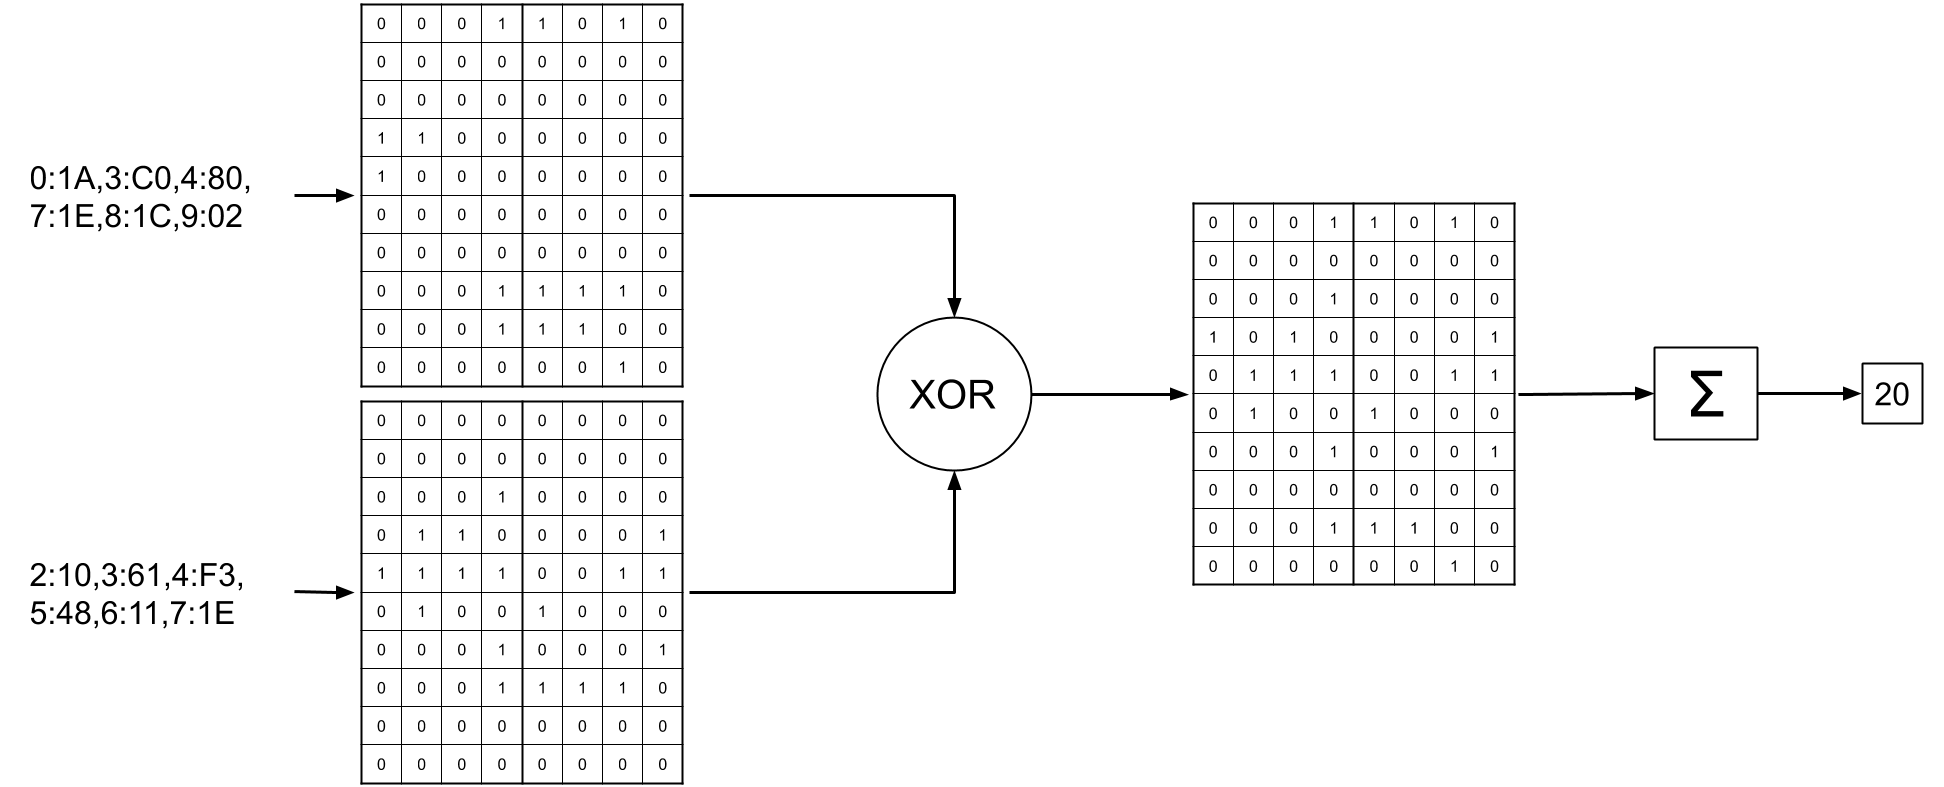
\includegraphics[width=0.95\linewidth]
    {Levenshtein/figuras/fig41.png}
    \caption{Cálculo de la distancia de Levenshtein}
    \label{fig:LevenDist}
\end{figure}

% Esto para cada entrada del diccionario -> se obtiene tabla simetrica de
% distancias respecto a la diagonal.
Podemos elaborar una lista con las distancias entre el \textit{target run} y 
todas las entradas del diccionario de forma que la componente \textit{"i"} sea 
la distancia de Levenshtein entre el \gls{SEU} a diagnosticar y la entrada 
\textit{"i"}. Acompañando a esta lista tendríamos otra en la que se encuentra la
información de las inyecciones. 

Por último, notar que al tratarse de distancias, se cumplen las propiedades
típicas de una distancia: 
\begin{center}
    \textit{D(i,i) == 0}

    \textit{D(i,j) == D(j,i)}
\end{center}

\section{Diagnóstico basado en la distancia de Levenshtein}
\label{sec:LevenCands}
% Explicar cómo se seleccionan los candidatos en base a las distancias calculadas
% y por qué se selecciona de esa manera y no de otra. En one note hay apuntes de
% esto
Una vez hayamos calculado las distancias de Levenshtein entre el \textit{target
run} y todas las entradas del dicionario y hayamos elaborado las dos listas
mencionadas tendremos todo lo necesario para llevar a cabo el diagnóstico con esta
primera versión de la técnica. 

Tal y como hemos explicado en el último párrafo del apartado \ref{ch:Levenshtein},
las entradas del diccionario cuyas inyecciones se encuentren más próximas a la
que habría probocado al \textit{target run} presentarán las menores distancias
hasta el mismo. Diagnósticar consiste en seleccionar estas entradas, las cuales
pasarán a llamarse \textit{"Candidatos"}.

Originalmente, el proceso que seguíamos para seleccionar candidatos consistía en
establecer una distancia de corte en función de las distancias máxima y mínima. El
corte se establecía según el porcentaje especificado del rango sobre el mínimo. De
esta forma, eran seleccionados todos runs cuya distancia era menor o igual que el
valor establecido:
% Ecuacion del porcentaje
\begin{equation}
    \label{eq:SeleccionPorcentaje}
    D(i) \leq tolerancia \times \frac{(max - min)}{100} + min
\end{equation}
Donde tolerancia establecía qué porcentaje del rango de distancias se toma. De 
esta forma, todos aquellos runs cuyas distancias cumplían la ecuación
\ref{eq:SeleccionPorcentaje} pasaban a ser candidatos.

% Problemas detectados con este sistema de selección.
El problema de este sistema es que no controlabamos cuántos candidatos
seleccionabamos en cada ocasión. Para valores de tolerancia de 1 a 5, se obtenían
cantidades de candidatos bastante dispares en los diseños de circuitos en que se
probó. Los causantes son valores de distancias aislados y alejados del resto, es
decir, un mínimo o un máximo aislado mucho menor o mayor que el resto
respectivamente. Esto proboca que el rango de distancias se alargue y se
concentren todas muy próximas al extremo, seleccionando bien muy pocos o bien
demasiados candidatos respectivamente.

% La version final... ordenar y coger los n primeros
Este problema puede solucionarse si se identifican y descartan estas distancias
antes de calcular el valor de corte, pero si analizamos bien, veremos que hay una 
solución mejor: ordenar la lista de distancias de menor a mayor y seleccionar las 
entradas correspondientes a las \textit{"n"} primeras distancias, siendo 
\textit{"n"} el número de candidatos que deseemos seleccionar, especificado como 
argumento de entrada.

\section{Resultados experimentales}
\label{sec:LevenResults}
Aunque se realizaron bastantes experimentos hasta llegar a la solución última de
seleccionar los \textit{"n"} primeros runs, hablaremos solo de aquellos resultados
correspondientes a la versión última de este algoritmo.

Para probar la técnica disponíamos de una serie de circuitos con sus respectivos
diccionarios de fallos. Algunos de estos eran exhaustivos, mientras que de otros,
debido al tamaño del circuito, solo diaponíamos de uno incompleto fruto de una
campaña de inyección de fallos aleatoria. Concretamente disponíamos de un
diccionario del 0'005\% de exhaustividad para el diseño de la \textit{FFT}, 0'87\%
para la \textit{UART} y 37'78\% para el \textit{FIR\_RI}.

Tanto estos diseños como el resto de circuitos que hemos empleado para las pruebas
%\cite{Triplelogic}

\subsection{Diccionarios exhaustivos}
\label{subsec:LevDicExhaust}
% Siempre aparece mínimo el correcto, a veces más debido a colisiones


\subsection{Diccionarios no exhaustivos}
\label{subsec:LevDicNoExhaust}


\endinput

%
\chapter{Inclusión de la distancia temporal en el algoritmo de selección de
candidatos}
\label{ch:Cycle}

% Explicar el concepto de la distancia temporal con algún ejemplo.
\lettrine[lraise=-0.1, lines=2, loversize=0.2]{L}{a} idea de implementar una
distancia basada en ciclos surge de la observación realizada en los resultados de
la distancia de Levenshtein (ver subsección \ref{subsec:LevDicNoExhaust}). La
también llamada \textit{"distancia de ciclos"} se calcula a partir del primer 
ciclo en que la inyección se manifiesta a la salida, a partir de ahora 
\textit{"first cycle"}. La distancia de ciclos se calcula como la diferencia 
entre el \textit{first cycle} del target run y el \textit{first cycle} de cada 
entrada del diccionario, pudiendo ser positiva, negativa o cero si el fallo del 
target run se manifiesta antes, despues o en el mismo ciclo que el de las 
entradas del diccionario.

% Decir las hipótesis realizadas para diagnosticar en base a la distancia de Cycle
    % Esta distancia no es nada sin la de levenshtein. Lev = 0 es que hemos i
    % terminado, cycle = 0 no implica Lev = 0
La hipótesis que realizamos basándonos en las observaciones y la cual aplicamos
para mejorar el diangóstico sería la siguiente:
\begin{hypothesis}\label{hyp:cycle}
    "La distancia temporal, definida como la diferencia entre los primeros ciclos
    en que se manifiestan dos inyecciones, guarda relación directa con la
    diferencia entre los ciclos de inyección de dichas inyecciones".
\end{hypothesis}

Puntualizar que, mientras una distancia de Levenshtein nula significa que 
producen el mismo fallo a la salida y por tanto, bien son el mismo \gls{SEU} o 
bien colisionan; una distancia temporal nula no implica que nos encontremos ante
la misma inyección. Se cumple que:
\begin{center}
    $D_{Levenshtein} = 0 \Rightarrow D_{ciclo} = 0$
\end{center}

% Explicar que la base de datos de distancias se genera de forma similar
% dist = first_cycle[i] - target_first_cycle
Para generar la lista de distancias de ciclo entre el target run y el resto del
diccionario primero leemos la información de ambos archivos tal y como
explicabamos en la sección \ref{sec:LevenDist}. Despues identificamos el primer
ciclo en que se manifiestan las inyecciones para cada entrada del diccionario.
Hacemos lo propio con el \gls{SEU} que estamos diagnosticando. La distancia de
ciclos se calcula como primer ciclo de la entrada menos primer ciclo del target
run. Se hace el cálculo para cada entrada del diccionario y se almacenan las
distancias temporales junto con las respectivas distancias de Levenshtein.

% Imagen ilustrativa cálculo de la distancia temporal
\begin{figure}[htbp]
    \centering
    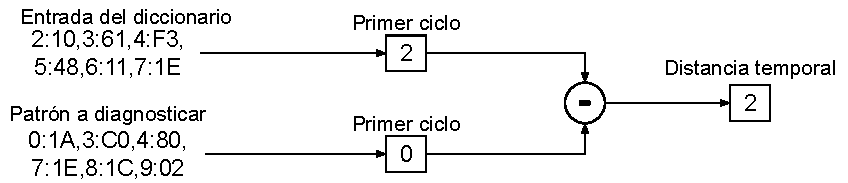
\includegraphics[width=0.95\linewidth]
    {Cycle/figuras/fig51.pdf}
    \caption{Cálculo de la distancia temporal}
    \label{fig:CycDist}
\end{figure}

% Decisiones tomada cuando el run es vacío y por qué
Al diagnosticar, suponemos que el target run presenta fallos a la salida, ya que
debe existir un error que detectar antes de saber que tenemos algo que
diagnosticar, por lo que siempre existirá primer ciclo para él. Esta afirmación no
es cierta para el resto de entradas del diccionario. Todas se corresponden con una
inyección, pero no todas producen errores a la salida. Esto se traduce en la
existencia de runs vacíos en el archivo \textit{"damages.csv"} y por tanto, en
entradas del diccionario a las cuales no se le puede asignar un \textit{first
cycle} de forma inmediata.

Cuando una inyección no se manifiesta a la salida puede deberse a tres razones
básicas:
% Solucion adoptada para esto
\begin{enumerate}
    \item El \gls{SEU} se produjo durante el reset, por lo que automáticamente se
        restaura el sistema.
    \item El \gls{SEU} no ha tenido tiempo suficiente para manifestarse a la
        salida.
    \item El \gls{SEU} esta localizado (FF, ciclo) en un sitio donde no produce
        fallos a la salida.
\end{enumerate}
Con la información que disponemos del propio diccionario, podemos identificar las
inyecciones que se han producido durante un reset del circuito y las que  se han
producido muy próxima al fin de su ejecución, no teniendo tiempo de manifestarse.

Aunque podríamos aproximar estos dos casos a primer ciclo cero y último
respectvamente, al final decidimos que lo mejor era descartar directamente los
runs vacíos como candidatos, ya que el target run siempre presenta fallos a la
salida y por tanto, en ningún caso puede corresponderse con una entrada del
diccionario vacía.

\section{Diagnóstico basado en la distancia temporal}
\label{sec:CycleCands}
% Explicar cómo se seleccionan los candidatos en base a las distancias calculadas
La selección de candidatos, en su versión final, la realizamos de la misma forma 
que para la distancie de Levenshtein con un ligero matiz. Las entradas del
diccionario se ordenan de menos a mayor según el valor absoluto de su distancia
temporal al target run. Una vez hecho esto, se seleccionan los \textit{"n"}
primeros.

El \gls{FF} de inyección de los candidatos seleccionados según la distancia
temporal no aporta información. Sin embargo, observamos cómo, en circuitos
simples, el ciclo donde se localiza el \gls{SEU} bajo diagnóstico coincide con 
la diferencia entre el ciclo de inyección del candidato y la distancia temporal 
que este presente hasta el target run. Para circuitos más grandes, con un mayor
número de biestables y que por tanto requieren ser ejecutados durante más ciclos
para que el diccionario presente las diferencias suficientes entre inyección e
inyección, observamos como este cálculo se aproxima bastante al valor del ciclo
real del target run. En la \textit{uart} por ejemplo, el margen de error oscila
en torno a los 1000 ciclos de los 37000 ciclos que componen cada ejecución.

Observamos además cómo el error cometido disminuye si lo hacemos con candidatos
que además dispongan de una distancia de Levenshtein relativamente baja.


\section{Fusión de las distancias temporal y de Levenshtein}
\label{sec:FusionLevenCycle}
% Puntos fuertes de cada algoritmo
El objetivo que perseguimos al fusionar las dos distancias es sacar partido de los
puntos fuertes de cada una de ellas.

Por un lado, la distancia de Levenshtein suele aproximarse más al registro e
incluso \gls{FF} correcto. Mientras que la distancia temporal resulta muy útil
para localizar temporalmente al \gls{SEU}.

% Explicar como se modifica el algotirmo para fusionar las dos distancias
El procedimiento que hemos seguido para diagnosticar conjuntamente con las dos
distancias consistía en calcular todas las distancias y agruparlas en una sola
lista, ordenar la lista de menor a mayor en función de la distancia de
Levenshtein y seleccionar los \textit{"n"} primeros.

% Cada candidato se muestra con las dos distancias auque sea seleccionado segun 
% una en concreto
Llegados a este punto, el algoritmo mostraba por pantalla, para cada candidato
seleccionado, su distancia de Levenshtein, su distancia de ciclo y la información
de su inyección. Además, dado que para nosotros esa información era conocida,
mostrabamos la localización correcta del \gls{SEU} a diagnosticar. Podíamos
comprobar cómo efectivamente, la inyección de los candidatos obtenido con la
distancia de Levenshtein podía ser corregida con la distancia temporal.

Más adelante, para la vesión final de la técnica, contenida en el capítulo
\ref{ch:CampanasIterativas}, veremos cómo hemos integrado el cómputo del ciclo de
inyección completamente en el algoritmo.

\section{Resultados experimentales}
\label{sec:CycleResults}
Dado que la distancia temporal no está lo suficientemente básada en la salida 
como para realizar un diagnóstico completo únicamente a partir de ella, es difícil
mostrar unos resultados experiementales de este algortimo aislado. Además, no fue
hasta más adelante, con la inclusión de dos aproximaciones más que aún faltan por
explicar, que empezamos a registrar resultados donde la distancia temporal 
intervenía.

Es por eso que a continuación vamos a ver sólo unos datos que se obtienen previos
a la fusión de las dos distancias.

\subsection{Diccionarios no exhaustivos}
\label{subsec:CycDicNoExhaust}
Dado que el diagnóstico con diccionarios exhaustivos se resuelve únicamente con la
distancia de Levenshtein, y esta investigación trata de desarrollar técnicas de
diagnóstico de \gls{SEU} con diccionarios incompletos, vamos a centarnos
únicamenrte en los resultados que se obtienen con estos últimos.

% Tabla de resultados solo con leven. 5 cands, 5% o menos, reg
\begin{table}[htbp]
    \ttabbox
    {\caption{Resultados experimentales. Distancia de ciclos. Dic.
    incompletos ($\leq5\%$)}
    \label{tab:LevenRes}}
    {
        \begin{tabular}{c|c c}
            \hline
            \rule[-8pt]{0pt}{22pt}{\bfseries{Diseños}}&{\bfseries{Registro}}
            &{\bfseries{\gls{FF}}} \\
            \hline
            \rule{0pt}{14pt}adder\_acum & 100 & 37\\
            counter & 100 & 63\\
            dual\_counter & 98 & 67\\
            fifo & 98 & 0\\
            fir\_ri (37'78\%) & 21 & 4\\
            pcm & 67 & 52\\
            shiftreg & 100 & 52\\
            simple\_fsm & 100 & 88\\
            uart (0'87\%) & 92 & 74\\
            \hline
        \end{tabular}
    }
\end{table}

Los experimentos a partir de los cuales se han obtenido los datos de la tabla se
han realizado de la misma forma que la explicada en el capítulo anterior
(ver \ref{subsec:LevDicNoExhaust}), y los números representan también el número de
veces de las 100 simuladas que se encuentra el Registro/FF correcto entre los
candidatos.

Observamos cómo efectivamente se tiene menos capacidad de diagnóstico para 
\gls{FF} con la distancia de ciclo. Parece que además el porcentaje de acierto
ronda en torno al 50\%, lo cual encaja con la hipótesis de que la ditancia
temporal no sirve más que para localizar el \gls{SEU} temporalmente, obteniendo
este nivel de acierto fruto del azar, aunque con excepciones.

Para el \textit{fifo} y el \textit{fir\_ri} el bajo nivel de acieto se explica
debido a una cantidad muy alta de colisiones. Además de los \textit{"n"} 
candidatos seleccionados hay muchos otros que son equidistantes a ellos y que no
se seleccionan, quedando atrás las inyecciones correctas a causa de las
colisiones.

Por el contrario, si que observamos circuitos donde se supera claramente la mitad
de aciertos. El caso de la máquina finita de estados se explica porque existen muy
pocos \gls{FF} donde seleccionar, por lo que es muy probable que uno de los
correctos se encuentre entre los candidatos. La \gls{UART} no tiene una
explicación tán sencilla. Puede deberse a la propia ejecución que está ejecutando.
Las zonas del circuito podrían estar activandose alternadamente por periodos, con
lo que al detectar los más próximos temporalmente, estaríamos seleccionando además
inyecciones a los mismos registros o incluso biestables.

\endinput

% 
\chapter{Técnicas de diagnóstico auxiliares}
\label{ch:TecnicasAuxiliares}

\lettrine[lraise=-0.1, lines=2, loversize=0.2]{}{}
% Explicar que se probaron otras distancias y que, como a veces seleccionan buenos
% candidatos que a Lev se le escapan, los algoritmos se han mantenido a modo de
% respaldo.
% Comentar que más adelante, cuando hablemos de las campañas iterativas, su fucion
% además es la de evitar posibles mínimos locales.


\section{Diagnóstico basado en el análisis de imágenes}
\label{sec:HuDist}
% Explicar el concepto. Diagnostico basado en la identificación de patrones con
% técnicas de reconocimientos de objetos en imágenes.
% Conversión de las entradas del diccionario en imágenes
% Explicar que son los momentos invariantes de Hu
% Calculo de distancias en base a los momentos de Hu. Modulo del vector.
% Explicar cómo se seleccionan los candidatos en base a las distancias calculadas


\section{Diagnóstico por coincidencias}
\label{sec:CoincDist}
% Explicar en que consiste
% Explicar cómo se calculan las distancias de coincidencia
% Explicar cómo se seleccionan los candidatos en base a las distancias calculadas


\section{Resultados experimentales}
\label{sec:CycleResults}
% Explicar, en lineas generales, los resultados que se obtienen al realizar una
% selección de candidatos ejecutando estos algoritmos por separado
% Decir que analizarán resultados más adelante.


\endinput

%
\chapter{Campañas iterativas a partir de los candidatos seleccionados}
\label{ch:CampanasIterativas}

% Explicar en qué consiste una campaña iterativa. Comentar que puede ser una buena
% solucion para cuando el diccionrio es extremadamente pequeño. -> Random sampling
% y a partir de ahi acotar
\lettrine[lraise=-0.1, lines=2, loversize=0.2]{L}{as} campañas iterativas serían
el recurso propuesto para diagnósticos que no encuentran candidatos a distancias
cero, es decir, cuando el diccionario no contiene al \gls{SEU} que queremos
diagnosticar. Esta técnica aplica para diccionarios incompletos, ya que un
diccionario completo siempre contendrá por definición al target run.

Esta técnica se emplea en situaciones en las que el diccionario es extremadamente 
pequeño pero sin llegar a perder completamente la capacidad de diagnóstico. El
concepto es sencillo. Se obtiene un diccionario incompleto del circuito mediante
inyecciones aleatorias (\textit{"Random Sampling"}), a partir de él, realizamos el
primer diagnóstico. Obtenemos una lista preliminar de candidatos a partir de la
cual extraemos la información necesaria para una siguiente inyección, que ya no 
será aleatoria, al menos en su mayoría. El proceso de obtención de diccionario,
diagnóstico, y obtención de un nuevo diccionario a partir del el cual volver a
diagnosticar puede repetirse tantas veces como sea necesario, finalizando con la
detección de al menos una inyección que colisione con el target run.

% Reducir enormemente el espacio de inyeccion restringiendo a un rango de ciclos,
% registros, todos los regs pero en un único ciclo, un solo FF pero un rango de
% ciclos, etc
Según la información de salida del algoritmo que selecciona los candidatos,
podemos realizar nuevas campañas desde distintos enfoques.
% LISTA POSIBLES TIPOS DE CAMPAÑA
    % Campaña enfocada en ciclos
    % Campaña enfocada en registros
    % Campaña enfocada en FF concretos
    % Combinación de las anteriores.
\begin{itemize}
    \item Campaña enfocada en ciclos: si la información de salida no deja duda
        sobre en qué ciclo se localiza el \gls{SEU}, podemos realizar una campaña
        de inyección de fallos en la que sólo inyectemos durante ese ciclo en
        concreto. El espacio total a inyectar se reduce al número de biestables, y
        la longitud de la simulación se divide por la cantidad de ciclos que
        componían cada ejecución.
    \item Campaña enfocada en registros: cuando la información de la salida apunta
        claramente a un registro o un conjunto de ellos, la campaña de inyección
        de fallos a realizar podría centrarse en inyectar esas zonas del circuito,
        reduciendo el espacio de inyección al descartar de la campaña el resto de
        registros del \gls{CUT}.
    \item Campaña enfocada en biestables: del mismo modo, podríamos inyectar
        \gls{FF} concretos del \gls{CUT} en todos los ciclos posibles.
    \item Combinación de las restricciones anteriores: si el circuito es tan
        grande que toda reducción del espacio de inyección es poca, podemos acotar
        la siguiente campaña combinando restricciones. Inyectar un registro
        durante un rango de ciclos, un ciclo pero un conjunto de \gls{FF}, etc.
\end{itemize}

% Comentar con qué formato sale la información para la siguiente campaña, siendo
% el usuario el que decide qué tipo de campaña realizar.
El código que selecciona y procesa los candidatos devuelve una lista de biestables
concretos, donde cada biestable va acompañado del número de veces que ha sido
seleccionado y de un rango de ciclos que se calcula en función de la distancia en
ciclos. También se indica el ciclo central del rango, siendo posible, cuando no
cabe ninguna duda, de que el rango sea un único ciclo. Por separado, se muestran,
de existir, las inyecciones del diccionario que producen exactamente el mismo
patrón de fallos.

Con esta información, es el usuario el que decide cuál de las 4 campañas descritas
aplicar, siendo una buena opción inyectar tal cual esos biestables en el rango de
ciclos que los acompañan. En cualquier caso, si la duración de la campaña lo
permite, realizar una campaña menos acotada evitará malos diagnósticos y mínimos
locales.

% MINIMOS LOCALES
% Explicar la posibilidad de llegar a un minimo local -> soluciones planteadas
    % El uso de los 4 algoritmos simultaneamente -> 4*n candidatos
    % Posibilidad de incluir además un set de inyecciones aleatorias en la
        % siguiente campaña
Alcanzar un mínimo local en este contexto sería como "seguir una pista falsa".
Corremos el peligro de caer en un mínimo local cuando el candidato que presenta la
menos de las distancias no apunta a donde debería. Esto es más probable conforme
reducimos la exhaustividad del diccionario. De esta forma, campaña tras campaña,
acotaríamos el espacio de inyección en torno a una zona que presenta aparentemente
menos distancia al taget run, pero en la que nunca detectaremos una colisión. 

Este problema se podría evitar aumentado el número de candidatos que seleccionamos
(\textit{"n"}) o tratando de acotar más progresivamente. Otra posibilidad es la
incluir inyecciones aleatoriamente en cada nueva campaña, de forma que se aumenten
las probabilidades de estimular la zona correcta si previamente esta no estaba
contenida en el diccionario.

Las características y puntos fuertes de cada técnica en particular también pueden
propiciar la caída en un mínimo local. Esta es otra razón por la que hemos
decidido mantener los cuatro algoritmos a la hora de extraer candidatos. El
objetivo es que, si uno de los algoritmos se ve especialmente influenciado por un
mínimo local, los otros tres incluyan candidatos en la campaña que pertenezcan a
otra zona del circuito. Como mencionamos en los resultados del capítulo anterior,
la distancia en ciclo cumple especialmente bien este objetivo al no tener
capacidad para diagnosticar espacialmente por sí sola.

\section{Obtención de la lista de candidatos}
\label{sec:Candidatos}
% Mencionar lo ya explicado anteriormente sobre el uso de los 4 algoritmos
% simultaneamente
% Seleccion de n candidatos de cada algoritmo
Primeramente leemos la información tanto de \textit{"dammages.csv"} como de 
\textit{"injections.csv"} y leemos el patrón de fallos a diagnosticar. En este
momento calculamos todas las distancias y agrupamos la información de las
distancias y las inyecciones en una lista. Tal y como hemos explicado para cada
distancia, realizamos la selección de los \textit{"n"} primeros candidatos con
cada una (máximo de $2 \times n$ como hemos comentado).

% Agrupacion de los candidatos en una sola lista (en el siguiente apartado
% explicamos cómo se procesa esta información)
Agrupamos los $4 \times n$ candidatos en una sola lista, manteniendo aún todas las
distancias para cada uno de ellos. A parir de este momento comenzamos a preparar
la información necesaria para la siguiente iteración.


\section{Extracción de la información para la siguiente campaña de inyección de
fallos}
\label{sec:InfoCampana}
% En este punto comprobamos si hay colision, es decir, si el diagnóstico ha
% terminado
Antes que nada, comprobamos si el diagnóstico
ha concluido, es decir, si alguno de los candidatos presenta distancia de
Levenshtein, ciclo y Hu igual a cero. Tanto en caso negativo como en positivo, 
procedemos a calcular la información de inyección recomendada para la siguiente 
campaña de inyección de fallos.

Aunque tras detectar candidatos a distancia cero pueda parecer que el diagnóstico
no puede mejorar, tenemos que tener en cuenta la posibilidad de encontrarnos ante
una colisión, por lo que la localización correcta del \gls{SEU} no sería esa.
Realizar una iteración extra y obtener una nueva lista de candidatos puede mejorar
el diagnóstico en este sentido, ya que podría llegar a localizar más inyecciones
que generen exactamente el mismo patrón, consiguiendo un diagnóstico más completo.

% Se agrupan los candidatos reg/FF repetidos y se calcula el rango de ciclos
La información recomendada para la siguiente inyección es de la forma que hemos
explicado hace un momento, biestables acompañados del número de veces que han sido
seleccionados y el rango de ciclos en el que podría estar, centrado en un ciclo
concreto e incluyendo márgenes de error. Para extraer esta información, primero
separamos las inyecciones de los candidatos en ciclo, registro y \gls{FF}. En este
punto disponemos de dos posibilidades, agrupar inyecciones por \gls{FF} o por
registros repetidos, realizando el recuento de cuántas veces se repiten. En 
nuestro caso, dado el alto porcentaje de acierto inicial, hemos decidido agrupar 
los candidatos repetidos por biestables.

Por último, recorremos de nuevo la lista de candidatos que contiene las
distancias calculando el rango de ciclos en los que el algoritmo selecciona cada
uno de ellos y estimando la posición central. Esta se calcula mediante la ecuación
\ref{eq:CicloCentral}, y el margen de error que compone el rango se ha establecido
como dos veces la distancia en ciclos para cada sentido a partir del ciclo central.

\begin{equation}
    \label{eq:CicloCentral}
    Ciclo\_Central = Ciclo\_de\_inyección - Distancia\_en\_ciclos
\end{equation}

% Como resultado se obtiene una lista con toda la informacion necesaria para
% realizar la siguiente campaña recomendada
Como resultado de este proceso obtenemos una lista con toda la información
necesaria para realizar la siguiente campaña de inyección de fallos. Esta
información se muestra con el siguiente formato:
\begin{center}
    [ciclo inferior, ciclo central, ciclo superior] \hfill :/ \hfill registro/
    \hfill \gls{FF} \hfill nº de repeticiones
\end{center}

Aunque esta
información tal cual se correspondería con la próxima campaña recomendada, aún
podemos decidir manualmente, tras observar los rangos de ciclos y la variedad de
registros o \gls{FF}, si realizaremos una campaña especialmente enfocada en alguna
parte del circuito tal y como hemos comentado anteriormente.


\section{Resultados experimentales}
\label{sec:IterResults}
% Validacion de los resultados sin necesidad de inyectar (porque conocemos de
% antemano la inyeccion correcta del target run)
Los experimentos realizados para validar esta técnica se basan en la siguiente
hipótesis:

% Hipotesis realizadas para validar de esta forma
\begin{hypothesis}\label{hyp:ResIter}
    "Si el espacio de inyección propuesto por el algoritmo es lo suficientemente
    pequeño como para realizar en él una campaña exhaustiva, y en en él se
    encuentra la inyección correcta; la siguiente campaña detectará al menos una
    colisión".
\end{hypothesis}

% Comentar la hipótesis. Conocemos la inyeccion real de target run.
Conociendo de antemano la inyección del \gls{SEU} que se quiere diagnosticar, se 
puede saber si el proceso iterativo terminará detectando colisiones o no.
Podemos pues ahorrarnos el proceso de inyección de cara a validar la técnica, ya
que los experimentos de diagnóstico se están realizando para conmutaciones lógicas
simuladas, y por tanto conocemos la información de la inyección. Esta información
nos permite tanto validar la técnica como saber de antemano cuál es la mejor
campaña que podemos aplicar dada la salida del algoritmo.

% Cuando diremos que las campañas iterativas serán exitosas.
Hemos fijado \textit{"n"} a 5. Esto hace un total de 20 candidatos (con un máximo
de 40) en caso de que no se repita ninguno. Si además tenemos en cuenta que el
algoritmo nos acota también el espacio de inyección temporalmente, podemos afirmar
que este es lo suficientemente pequeño como para aplicar una campaña de inyección
de fallos exhaustiva.

Por supuesto, aún tenemos libertad para decidir a qué ciclos aplicamos la campaña,
pudiendo ampliarlos o reducirlos, y si la aplicamos a biestables concretos o si 
por el contrario inyectamos en todos los \gls{FF} de los registros
seleccionados. Hemos programado un código que analiza la salida del algoritmo, la
compara con la información de la inyección y predice el resultado que se obtendría
al realizar realmente las campañas de inyección de fallos. Las posibles salidas de
este código son:
\begin{itemize}
    \item \textit{"Next campaign will fail"}: en caso de que entre los candidatos 
        no se encuentre ni el \gls{FF}, ni el registro, ni el ciclo correcto.
    \item \textit{"Will need more than one iteration to hit the target"}: cuando
        entre los candidatos se encuentra el \gls{FF} correcto, pero el ciclo está
        fuera del rango. Los nuevos candidatos extraidos del diccionario resultado
        de la siguiente inyección afinarán la predicción temporal. Una campaña
        exhaustiva para los \gls{FF} seleccionados no acotada temporalmente solo
        necesitaría una campaña extra para colisionar.
    \item "If next campaign is oriented to registers, will hit the target": tanto
        el registro como el ciclo correcto están en el espacio de inyección
        acotado, pero el biestable concreto no aparece. Si la campaña la enfocamos
        a registros, sin concretar en cuáles de sus biestables se inyecta,
        localizará al target run.
    \item "Next campaign will hit the target": tanto ciclo, como registro, como
        biestable están en el espacio de inyección seleccionado. Las campañas
        iterativas finalizarían en la siguiente iteración.
    \item "Next campaign will contain only right cycle": sólo una campaña acotada
        temporalmente aseguraría mejorar el diagnóstico en la siguiente iteración.
    \item "Will need a register oriented campaign and more than one iteration": ni
        ciclo ni biestable correcto se encuentran en el espacio de inyección
        seleccionado. A base de iterar podría mejorar el diagnóstico temporal
        empleando la información de las nuevas distancias en ciclo, pero sería
        necesario no enfocar las campañas a biestables concretos.
\end{itemize}

Evidentemente, en una aplicación real no dispondríamos de la información correcta
de la inyección, por lo que no se sabría qué tipo de campaña realizar en la
próxima iteración para mejorar el diagnóstico. La información del número de veces
que se repite cada biestable entre los candidatos puede orientarnos a la hora de
saber si realmente el \gls{FF} correcto se encuentra entre ellos o no. Aún
así, es posible que se necesiten varios intentos de selección de tipo de campaña
en caso de que, debido al gran tamaño inicial del espacio de inyección, sea
necesario acotar lo máximo posible.

% Resultados (ver correo, que ahí hago el resumen)
En líneas generales, los resultados muestran como el candidato que se repite un
mayor número de veces es el que apunta al biestable correcto si la diferencia
de repeticiones respecto al resto es notable. A pasar de lo claro
que sea este resultado, se debe inyectar también en el resto de candidatos, en caso
de que no se haya detectado colisión, para evitar caer en un mínimo local.

He seleccionado los resultados más significativos de todos los experimentos
realizados, mostrando algún ejemplo para cada posible caso de los anteriormente
enumerados.

\begin{lstlisting}[language=,caption={Adder Acum: diagnóstico de la inyección
11:/i\_valor\_acum/10 }, breaklines=true, label=s:adder0]
[-62, 11, 84]  :/	i_valor_acum/	10	x8
[-77, 11, 99]	:/	i_valor_acum/	15	x2
[-58, 11, 80]	:/	i_valor_acum/	5	x2
[11, 11, 11]	:/	i_valor_acum/	9	x1
[11, 11, 11]	:/	i_valor_acum/	17	x1
[10, 11, 12]	:/	i_valor_acum/	16	x1
[9, 11, 13]	:/	i_valor_acum/	8	x2
[8, 11, 14]	:/	i_valor_acum/	6	x1
[5, 11, 17]	:/	i_valor_acum/	1	x1
[5, 11, 17]	:/	i_valor_acum/	0	x1

11	:/	i_valor_acum/	10
Next campaign will hit the target
\end{lstlisting}

En la salida \ref{s:adder0} no se produce colisión, pero en la información de 
salida vemos que todos los ciclos centrales apuntan al ciclo 11 (el correcto) y 
que 8 de los 20 candidatos apuntan hacia el \gls{FF} correcto.
Se podría realizar una campaña de una única inyección al (11, i\_valor\_acum/10) 
para comprobar que efectivamente, esa localización produce el mismo patrón de
fallos a la salida que el target run, o se podría simplemente lanzar la siguiente
campaña sugerida al completo.

\begin{lstlisting}[language=,caption={Adder Acum: diagnóstico de la inyección
63:/i\_valor\_acum/4},breaklines=true, label=s:adder64]
Iterative campaign its over. Colision founded:
63	:/	i_valor_acum/	4

To assure the result, this is the sugested campaign:

[35, 63, 91]	:/	i_valor_acum/	4	x8
[27, 63, 99]	:/	i_valor_acum/	15	x1
[28, 63, 98]	:/	i_valor_acum/	13	x1
[63, 63, 63]	:/	i_valor_acum/	0	x1
[63, 63, 63]	:/	i_valor_acum/	6	x2
[63, 63, 63]	:/	i_valor_acum/	17	x1
[62, 63, 64]	:/	i_valor_acum/	8	x2
[62, 63, 64]	:/	i_valor_acum/	9	x1
[50, 63, 76]	:/	i_valor_acum/	14	x1
[59, 63, 67]	:/	i_valor_acum/	10	x1

63	:/	i_valor_acum/	4
Next campaign will hit the target
\end{lstlisting}

La salida \ref{s:adder64} ha detectado una colisión, que además sabemos es la
correcta. La información de la campaña sugerida para afianzar los resultados
apunta además al ciclo y registro correctos en su mayoría. Este es el mejor
resultado que se puede conseguir.

\begin{lstlisting}[language=,caption={Dual Counter: diagnóstico de la inyección
187:/counter1/reg\_i/5},breaklines=true, label=s:dcounter59]
[26, 187, 348]	:/	counter1/reg_i/	5	x16
[186, 187, 188]	:/	counter1/reg_i/	4	x2
[186, 187, 188]	:/	counter1/reg_i/	1	x2
[182, 187, 192]	:/	counter1/reg_i/	0	x1
[182, 187, 192]	:/	counter1/reg_i/	2	x1
[67, 187, 307]	:/	counter1/reg_i/	7	x2
[73, 187, 301]	:/	counter1/reg_i/	3	x1

187	:/	counter1/reg_i/	5
Next campaign will hit the target
\end{lstlisting}

El resultado de la salida \ref{s:dcounter59} es idéntico al resultado
\ref{s:adder0}, se aciertan ciclo y biestable correctos, con el valor añadido de
que este circuito tiene más de un registro.

\begin{lstlisting}[language=,caption={Dual Counter: diagnóstico de la inyección
157:/counter0/reg\_i/4},breaklines=true, label=s:dcounter29]
Iterative campaign its over. Colision founded:
27	:/	counter0/reg_i/	4
121	:/	counter0/reg_i/	4
159	:/	counter0/reg_i/	4
161	:/	counter0/reg_i/	4
223	:/	counter0/reg_i/	4
231	:/	counter0/reg_i/	4
251	:/	counter0/reg_i/	4

To assure the result, this is the sugested campaign:

[27, 150, 251]	:/	counter0/reg_i/	4	x16
[14, 14, 14]	:/	counter0/reg_i/	1	x1
[39, 39, 39]	:/	counter0/reg_i/	2	x1
[53, 57, 63]	:/	counter0/reg_i/	5	x6
[54, 63, 70]	:/	counter0/reg_i/	0	x3
[68, 68, 68]	:/	counter0/reg_i/	3	x1
[12, 264, 516]	:/	counter1/reg_i/	0	x5
[86, 86, 86]	:/	counter0/reg_i/	6	x1

157	:/	counter0/reg_i/	4
Next campaign will hit the target
\end{lstlisting}

La salida \ref{s:dcounter29} es un ejemplo de campaña finalizada en múltiples
colisiones. El diagnóstico termina pero no se sabe con certeza la localización del
\gls{SEU}. De hecho, todas las colisiones apuntan al biestable correcto pero entre
ellas no se encuentra la localización real. Una campaña extra, como hemos
explicado, mejoraría los resultados al encontrar más colisiones, estando ahora sí,
la localización correcta entre ellas.

\begin{lstlisting}[language=,caption={PCM: diagnóstico de la inyección
31:/I2S\_IN\_1/DATA\_L/1},breaklines=true, label=s:pcm59]
Iterative campaign its over. Colision founded:
9	:/	I2S_IN_1/DATA_L/	1
10	:/	I2S_IN_1/DATA_L/	1
11	:/	I2S_IN_1/DATA_L/	1
12	:/	I2S_IN_1/DATA_L/	1
13	:/	I2S_IN_1/DATA_L/	1
14	:/	I2S_IN_1/DATA_L/	1
15	:/	I2S_IN_1/DATA_L/	1
16	:/	I2S_IN_1/DATA_L/	1
17	:/	I2S_IN_1/DATA_L/	1
18	:/	I2S_IN_1/DATA_L/	1

To assure the result, this is the sugested campaign:

[9, 13, 18]	:/	I2S_IN_1/DATA_L/	1	x36
[12, 14, 15]	:/	CLK_96k/s_counter_lr/	1	x4

31	:/	I2S_IN_1/DATA_L/	1
Will need more than one iteration to hit the target
\end{lstlisting}

En la salida \ref{s:pcm59} volvemos a tener colisión múltiple. Esta vez, la 
campaña sugerida apunta por mayoría absoluta al FF correcto, pero el ciclo se 
encuentra fuera del rango. Las distancias temporales de los nuevos candidatos tras
una inyección extra es posible que nos reorienten el rango de ciclos, pero dado 
que existen colisiones, en un caso real no realizaríamos el mínimo de dos campañas
más que se necesitarían para encontrar primero el ciclo correcto y luego
inyectarlo.

\begin{lstlisting}[language=,caption={FIFO: diagnóstico de la inyección
3:/Memory\_149\_25},breaklines=true, label=s:fifo13]
Iterative campaign its over. Colision founded:
3	:/	Memory_1_6
3	:/	Memory_1_10
3	:/	Memory_1_27
3	:/	Memory_2_12
3	:/	Memory_2_26
3	:/	Memory_4_15
3	:/	Memory_4_28
3	:/	Memory_5_11
3	:/	Memory_5_12
3	:/	Memory_5_20

To assure the result, this is the sugested campaign:

[3, 3, 3]	:/	Memory_1_6	x3
[3, 3, 3]	:/	Memory_1_10	x3
[3, 3, 3]	:/	Memory_1_27	x3
[3, 3, 3]	:/	Memory_2_12	x3
[3, 3, 3]	:/	Memory_2_26	x3
[3, 3, 3]	:/	Memory_4_15	x3
[3, 3, 3]	:/	Memory_4_28	x3
[3, 3, 3]	:/	Memory_5_11	x3
[0, 3, 6]	:/	Memory_5_12	x4
[3, 3, 3]	:/	Memory_5_20	x3
[0, 3, 6]	:/	Memory_0_2	x1
[0, 3, 6]	:/	Memory_1_13	x1
[0, 3, 6]	:/	Memory_2_8	x1
[0, 3, 6]	:/	Memory_2_22	x1
[0, 3, 6]	:/	Memory_3_6	x1
[0, 3, 6]	:/	Memory_3_11	x1
[0, 3, 6]	:/	Memory_3_16	x1
[0, 3, 6]	:/	Memory_4_16	x1
[0, 3, 6]	:/	Memory_6_11	x1

3	:/	Memory_149_25
Next campaign will contain only right cycle
\end{lstlisting}

Otra situación extra de colisión múltiple se produce en la salida \ref{s:fifo13}.
Todos los candidatos de la campaña sugerida están de acuerdo en el ciclo, el cual
resulta ser el correcto. Se podría realizar una inyección abierta a todo el 
circuito pero centrada únicamente en ese ciclo con tal de detectar otras posibles
colisiones que completen aún más el diagnóstico. Notar que son tantas las
colisiones, que se han seleccionado el máximo impuesto de 40 candidatos y el
target run no es uno de ellos.

\begin{lstlisting}[language=,caption={UART: diagnóstico de la inyección
5804:/uart\_i/uart\_rx\_i/rx\_data/7},breaklines=true, label=s:uart5]
Iterative campaign its over. Colision founded:
8426	:/	uart_i/uart_rx_i/rx_data/	1
6131	:/	uart_i/uart_rx_i/rx_data/	6
6750	:/	uart_i/uart_rx_i/rx_data/	5
7210	:/	uart_i/uart_rx_i/rx_data/	4
6407	:/	uart_i/uart_rx_i/rx_data/	6
9079	:/	uart_i/uart_rx_i/rx_data/	0
6453	:/	uart_i/uart_rx_i/rx_data/	6
6864	:/	uart_i/uart_rx_i/rx_data/	5
8470	:/	uart_i/uart_rx_i/rx_data/	1
6172	:/	uart_i/uart_rx_i/rx_data/	6

To assure the result, this is the sugested campaign:

[8426, 8444, 8470]	:/	uart_i/uart_rx_i/rx_data/	1	x5
[6131, 6273, 6453]	:/	uart_i/uart_rx_i/rx_data/	6	x9
[6750, 6807, 6864]	:/	uart_i/uart_rx_i/rx_data/	5	x4
[7210, 7210, 7210]	:/	uart_i/uart_rx_i/rx_data/	4	x2
[9079, 9079, 9079]	:/	uart_i/uart_rx_i/rx_data/	0	x2
[1146, 5118, 9564]	:/	uart_i/uart_tx_i/tx_bit_count/	1	x13
[7014, 7782, 8550]	:/	uart_i/uart_rx_i/rx_bit_count/	2	x2
[4061, 9498, 14969]	:/	uart_i/uart_rx_i/	rx_pstate_FSM_FFd2	x2
[6483, 6969, 7455]	:/	uart_i/uart_rx_i/rx_bit_count/	1	x1

5804	:/	uart_i/uart_rx_i/rx_data/	7
\end{lstlisting}

La salida \ref{s:uart5} es previa a que programáramos el código que predice los
resultados de la siguiente campaña, por eso no se muestra la última línea como es
habitual. Tras analizar muchas salidas de este tipo de experimentos, este es el 
peor diagnóstico que he encontrado, y aún así detecta múltiples colisiones, 
todas apuntando al registro correcto aunque en diferentes biestables, sin ser el
correcto uno de ellos. Entre la información de la campaña sugerida no encontramos 
el ciclo correcto, ni el \gls{FF} correcto (realmente el ciclo correcto sí que se
encuentra entre los rangos, pero al no ir acompañando al registro correcto,
consideramos que no aparece). El \gls{FF} más votado se encuentra en un registro 
diferente (mínimo local), pero aún así, el registro correcto es votado 22 veces en
total frente a las 18 restantes. Adicionalmente, el registro erróneo más votado, 
está centrado muy aproximadamente alrededor del ciclo correcto. Si no hubieran 
existido colisiones, incluso en estas condiciones, con un poco de atención
podríamos haber detectado estas pistas y programado una nueva campaña enfocada al
registro y rango de ciclos correcto.

\begin{lstlisting}[language=,caption={UART: diagnóstico de la inyección
9179:/uart\_i/uart\_clk\_cnt/2},breaklines=true, label=s:uart6]
Iterative campaign its over. Colision founded:
10180	:/	uart_i/uart_clk_cnt/	2
10153	:/	uart_i/uart_clk_cnt/	2
10327	:/	uart_i/uart_clk_cnt/	2
9287	:/	uart_i/uart_clk_cnt/	2
9954	:/	uart_i/uart_clk_cnt/	2
10270	:/	uart_i/uart_clk_cnt/	2
10216	:/	uart_i/uart_clk_cnt/	2

To assure the result, this is the sugested campaign:

[147, 9487, 15662]	:/	uart_i/uart_clk_cnt/	2	x34

9179	:/	uart_i/uart_clk_cnt/	2
Next campaign will hit the target
\end{lstlisting}

Por último, la salida \ref{s:uart6} muestra un nuevo caso de colisión múltiple
entre los candidatos, con la diferencia de que todas apuntan por unanimidad al
biestable correcto, como el resto de la campaña sugerida. La localización temporal 
exacta no se encuentra entre los candidatos, pero si en el rango de ciclos
propuesto. Respecto al rango de ciclos, comentar que, al incluirle un margen de
seguridad de el doble de la distancia en ciclo máxima para cada sentido, que hacen
un rango total de cuatro veces la distancia máxima, este abarca prácticamente todo
el espacio de inyección. Podemos notar que el ciclo central se aproxima mucho al
ciclo correcto. Una buena campaña para detectar más colisiones podría ser
inyectar ese biestable en todos los ciclos de la ejecución.

% Decir que de todos los diccionarios son del 5% o menos, y que de los que
% originalmente eran ya incompleros, se ha eliminado el target run, siendo
% imposible que lo detecten a la salida en la primera selección de candidatos.
Cabe destacar que los diccionarios presentaban una exhaustividad del 5\%, pero
sobre todo, que de aquellos originalmente no exhaustivos se han eliminado las
entradas correspondientes a los 100 \gls{SEU} que se estaban diagnosticando,
explicando que en ninguna de las pruebas se haya detectado a la primera la
colisión correcta.

% Hablar de cuándo se va perdiendo la capacidad de diagnóstico conforme se va
% reduciendo la exhaustividad del diciconario
% Decir que no es lo mismo un diccionario del 1% para el counter que uno del 0'87%
% para la uart porque el núemro de entradas del primer caso es ridículo
Intentos de reducir aún más tanto los diccionarios completos como los diccionarios 
originalmente incompletos demostraron que la reducción afecta más a aquellos
diccionarios que originalmente eran de por sí muy pequeños. Esto se debe a que,
para el \textit{adder\_acum} por ejemplo, las 2000 entradas del diccionario
exhaustivo original se traducen en 100 entadas para el diccionario reducido al
5\%. Reducirlo al 1\% significaría diagnosticar con un diccionario de 20 muestras,
que lo hace estadísticamente insuficiente.

Sin embargo, en circuitos grandes como la \textit{uart}, el 0'87\% de
exhaustividad inicial se traduce en un diccionario de 16496 entradas. Reducirlo al
5\%, resultando en un diccionario exhaustivo al 0'04\%, no elimina completamente
nuestra capacidad de diagnóstico.

\endinput

%
\chapter{Aplicación de la técnica sobre diseños reales}
\label{ch:RealDesign}

\lettrine[lraise=-0.1, lines=2, loversize=0.2]{}{}
% Para validar la técnica, se ha probado con:

\section{Edelweis creo}
\label{sec:EdelweiCreo}
% Exponer los resultados optenidos para este diseño


\section{8061 o algo así}
\label{sec:8061}


\endinput

%
\chapter{Distancia en flip-flops. Mejora de la ditancia temporal}
\label{ch:FFdist}

\lettrine[lraise=-0.1, lines=2, loversize=0.2]{}{}
% Explicar el concepto de distancia en FF

% Explicar como se calcula la distancia en FF

\section{Inclusión de la distancia en flip-flops en el algoritmo}
\label{sec:FusionFF}
% Explicar como se modifica el algoritmo para incluir la distancia en FF.


\section{Resultados experimentales}
\label{sec:FFResults}


\subsection{Diccionarios exhaustivos}
\label{subsec:FFDicExhaust}


\subsection{Diccionarios no exhaustivos}
\label{subsec:FFDicNoExhaust}




\endinput

%
\chapter{Conclusiones y trabajos futuros}
\label{ch:FFdist}
% Las conclusiones en formato:
    % Se ha hecho X, Y, y funciona muy bien.
    % Se ha visto que ocurre A, B, C

\section{Conclusiones}
\label{sec:Conclusiones}
El propósito de esta investigación era desarrollar técnicas de diagnóstico de
\gls{SEU} utilizando diccionario de fallos incompletos. Para ello, partíamos de la
hipótesis \ref{hyp:inicial}, marcando la línea de investigación en encontrar una
métrica adecuada que permita sacar partido de las similitudes en los patrones que
generan dos conmutaciones lógicas próximas entre sí.

Hemos realizado experimentos en los que se diagnosticaba aplicando métricas cuyos
enfoques eran diferentes, todos ellos devolviendo unos resultados muy buenos.
Además, hemos establecido las bases de una técnica de diagnóstico consistente en
la realización de numerosas iteraciones de \textit{"Campaña de inyección de 
fallos para generar un diccionario de fallos"}, \textit{"Diagnóstico empleando el
diccionario de fallos obtenido"}, \textit{"Extracción de candidatos que acoten el
espacio de inyección"}, con la cuál hemos podido realizar diagnósticos exitosos 
con diccionarios de fallos muy incompletos en circuitos de grandes dimensiones.
Además, observamos como en muchas ocasiones, el diagnóstico se resuelve con la
campaña inicial, ya que los candidatos obtenidos no dejan duda.

Se ha propuesto además que siempre se realice una campaña extra tras finalizar el
diagnóstico, ya que los resultados apuntan a que iteraciones extras obtendrían, de
darse el caso, otras colisiones extras que enriquecerían el diagnóstico.

La técnica de campañas iterativas puede llevarnos hacia un mínimo local donde no
se encuentre el \gls{SEU} bajo diagnóstico, fallando su misión. Hemos propuesto
soluciones a este problema tales como la inclusión de inyecciones aleatorias en
cada iteración.

Hemos comprobado que la distancia temporal es especialmente útil para localizar
temporalmente el \gls{SEU} bajo diagnóstico. Para circuitos grandes, con
diccionarios muy reducidos, la exactitud de la distancia en ciclos se reduce, pero
los resultados demuestran que es capaz de acotar bastante la localización temporal
del \gls{SEU}.

La distancia de Levenshtein funciona especialmente bien como métrica de
diagnóstico. Hemos comprobado que a distancias de Levenshtein bajas, el cálculo de
ciclo realizado con la distancia temporal (ecuación \ref{eq:CicloCentral}) mejora,
aunque no es un requisito imprescindible para que este cálculo funcione con
exactitud.

% Conclusion sobre la perdida de diagnóstico con la exhaustividad:
    % Mas que exhaustividad, importa el número de entradas del diccionario
    % Se observa como la capacidad de diagnóstico se pierde progresivamente,
        % aunque por falta de experimentos no se puede asegurar en todos los
        % casos.
Los experimentos encaminados a determinar cuándo se pierde la capacidad de
diagnóstico sobre un circuito a base de reducir progresivamente la exhaustividad
del diccionario muestran que ésta no se pierde instantáneamente. Primero perdemos
la capacidad de localizar el biestable exacto, y posteriormente se van encontrando
más dificultades para determinar el registro donde se localiza el \gls{SEU},
siendo la capacidad de diagnóstico temporal lo último que se pierde. Es en este
punto de pérdida total donde deja de tener potencial de diagnóstico completo la
técnica iterativa, ya que hasta entonces, existirán campañas que mejoren el
resultado.

El hecho de que el primer intento de encontrar una distancia útil para diagnóstico
haya resultado muy bien, nos lleva a pensar que podrían existir muchas otras
métricas aún por explorar y que funcionen incluso mejor.
Podemos concluir la investigación afirmando que estas técnicas tienen capacidad de
diagnóstico con diccionarios de fallos incompletos; especialmente la técnica de 
campañas iterativas, la cual mantiene capacidad de diagnóstico incluso con 
diccionarios de fallos muy incompletos.

\section{Trabajos futuros}
\label{sec:TrabajosFuturos}
% Mejora: tabla dispersa para optimizar memoria
% Realizar el programa en C para acelerar el proceso
Las mejoras más inmediatas que se podrían realizar sobre la técnica son
optimizaciones computacionales. El código esta realizado completamente en Python,
por ser un lenguaje de programación con el que se hacen scripts muy rápidamente.
Traducir el lenguaje a código C reduciría significativamente el coste
computacional y los tiempos de cómputo.

Para optimizar el uso de la memoria, se podría reemplazar la forma de almacenar
los daños de cada entrada del diccionario por tablas dispersas.

% Aplicar la técnica en circuitos de mayor complejidad: edelweiss y 8051.
% Realizar experimentos reales, probar la técnica bajo radiación
Como trabajo futuro más inmediato, se podría aplicar la técnica a circuitos de
mayor extensión. Además sería interesante aplicar la técnica en circuitos tras
realizarles tests de radiación.

Por último, se podrían investigar otras formas de explotar las similitudes
existentes entre patrones cercanos.

\subsection{Otras técnicas de tratamiento de imágenes}
\label{subsec:OtrasTecnicasImag}
% Decir que existen otras muchas opciones para la localización de SEU empleando
% técnicas de diagnóstico de imágenes aún por explorar
El campo de la percepción por ordenador está muy desarrollado actualmente y avanza
muy rápido. Sería interesante explorar qué otras opciones existen para
diagnosticar basándonos en el tratamiento de imágenes.

% Estudiar otras formas mejores de indentificar patrones en imágenes para este
% caso

% Mencionar algunos ejemplos

% Mencionar avances del deep learning en el campo de la percepción que podrían
% impulsar el diagnóstico por esta vía.
Además, el \textit{deep learning} está experimentando grandes avances que podrían ser
aplicados para entrenar una red neuronal capaz de localizar un \gls{SEU} del
circuito para la que se le ha entrenado.


\subsection{Distancia en flip-flops. Mejora de la distancia temporal}
\label{subsec:FFdist}
Una posible mejora del diagnóstico, basada en la topología del circuito, puede ser
la que hemos llamado \textit{"Distancia en FF"}.

% Explicar el concepto de distancia en FF
La distancia en \gls{FF} de un biestable a otro sería el número mínimo de ciclos
de reloj que tomaría propagar un \gls{SEU} de uno a otro. Esta distancia puede
verse afectada por la dirección: 

\begin{center}
    $D(A-B) \neq D(B-A)$
\end{center}

Calculamos que esta distancia puede ser útil para afinar el diagnóstico una vez ya
se haya acotado lo suficiente al \gls{SEU}.

% Explicar como se calcula la distancia en FF
Para calcular la distancia en FF habría que contar cuántos elementos de lógica
combinacional separan dos biestables. Esto podría realizarse empleando la suite de 
Yosys por ejemplo \cite{YOSYS}.

\endinput

%
%\chapter{Referencias}
\label{ch:Referencias}
% Aplicacion de la técnica al diseño de circuitos resistentes a radiacion



\endinput

%

%%%%%%%%%%%%%%%%%%%%%%%%%%%%%%%%%%%%%%%%%%%%%%%%%%%%%%%%%%%%%%%%%%%%%%%%%%%%%%%
%%%%%%%%%%%%%%%%%%%%%%%%%%%%%%%%%%%%%%%%%%%%%%%%%%%%%%%%%%%%%%%%%%%%%%%%%%%%%%%
%%%%%%% Esto aún no lo he investigado, tengo que ver como va
%%%%%%%%%%%%%%%%%%%%%%%%%%%%%%%%%%%%%%%%%%%%%%%%%%%%%%%%%%%%%%%%%%%%%%%%%%%%%%%
%%%%%%%%%%%%%%%%%%%%%%%%%%%%%%%%%%%%%%%%%%%%%%%%%%%%%%%%%%%%%%%%%%%%%%%%%%%%%%%
%%%%%%% Apéndices
%%:Empezamos con los apéndices, que irían en uno o más ficheros. Es necesario incluir estos ficheros entre el entorno \begin{appendices}....\end{appendices} debido a que se ha deseado utilizar un formato diferente para el título de los apéndices, incluyendo la palabra apéndice, para la numeración de los apéndices, alfabético, y para las cabeceras de las páginas.
%
% \begin{appendices}
%
% % !TEX root =../LibroTipoETSI.tex



%APENDICE A
\chapter{Sobre  \LaTeX}\LABAPEN{ApA}
{Este es un ejemplo de apéndices, el texto es únicamente relleno, para que el lector pueda observar cómo se utiliza}
%%%%%%%%%%%%%%%%%
\section{Ventajas de \LaTeX}

El gusto por el \LaTeX\ depende de la forma de trabajar de cada uno. La principal virtud es la facilidad de formatear cualquier texto y la robustez. Incluir títulos, referencias es inmediato.
%\Blindtext
%\lipsum
Las ecuaciones quedan estupendamente, como puede verse en \EQ{Ap1}
\begin{equation}\LABEQ{Ap1}
x_{1}=x_{2}.
\end{equation}


\section{Inconvenientes}
%\Blindtext
El principal inconveniente de \LaTeX\ radica en la necesidad de aprender un conjunto de comandos para generar los elementos que queremos. Cuando se está acostumbrado a un entorno ``como lo escribo se obtiene'', a veces resulta difícil dar el salto a ``ver'' que es lo que se va a obtener con un determinado comando. 

Por otro lado, en general será muy complicado cambiar el formato para desviarnos de la idea original de sus creadores. No es imposible, pero sí muy difícil. Por ejemplo, con la sentencia siguiente:
 
\begin{lstlisting}[language=,caption={Escritura de una ecuación}, breaklines=true, label=prgA1-01]
\begin{equation}\LABEQ{Ap2}
x_{1}=x_{2}
\end{equation}
\end{lstlisting}
obtenemos:
\begin{equation}\LABEQ{Ap2}
x_{1}=x_{2}
\end{equation}
Esto será siempre así. Aunque, tal vez, esto podría ser una ventaja y no un incoonveniente.

Para una discusión similar sobre el Word\tsp{\textregistered}, ver \APEN{ApB}.
%\Blindtext


%%%%%%%%%%%%%%%%%%%%%%%%%%%%%%%%%%%%%%%
%APENDICE B
\chapter{Sobre Microsoft Word\tsp{\textregistered}}\LABAPEN{ApB}

\section{Ventajas del Word\tsp{\textregistered}}
La ventaja mayor del Word\tsp{\textregistered} es que permite configurar el formato muy fácilmente. Para las ecuaciones,
\begin{equation}
x_{1}=x_{2},
\end{equation}
tradicionalmente ha proporcionado pésima presentación. Sin embargo, el software adicional Mathtype\tsp{\textregistered} solventó este problema, incluyendo una apariencia muy profesional y cuidada. Incluso permitía utilizar un estilo similar al \LaTeX\xspace. Además, aunque el Word\tsp{\textregistered} incluye sus propios atajos para escribir ecuaciones,  Mathtype\tsp{\textregistered} admite también escritura \LaTeX\xspace. En las últimas versiones de Word\tsp{\textregistered}, sin embargo, el formato de ecuaciones está muy cuidado, con un aspecto similar al de \LaTeX.


\section{Inconvenientes de Word\tsp{\textregistered}}
Trabajar con títulos, referencias cruzadas e índices es un engorro, por no decir nada sobre la creación de una tabla de contenidos. Resulta muy frecuente que alguna referencia quede pérdida o huérfana y aparezca un mensaje en negrita indicando que  no se encuentra. 

Los estilos permiten trabajar bien definiendo la apariencia, pero también puede desembocar en un descontrolado incremento de los mismos. Además, es muy probable que Word\tsp{\textregistered} se quede colgado, sobre todo al trabajar con copiar y pegar de otros textos y cuando se utilizan ficheros de gran extensión, como es el caso de un libro.

%\end{equation}
 
%
% \end{appendices}

%%%%%%%%%%%%%%%%%%%%%%%%%%%%%%%%%%%%%%
%%%%%%%%%%%%%%%%%%%%%%%%%%%%%%%%%%%%%%
%:Empieza todo lo que no constituye el cuerpo en si del libro. Todo lo que va detrás
\backmatter

%:Indice de figuras, coméntese las siguientes líneas si no se desea
\cleardoublepage
\phantomsection

%:Para añadir una línea en blanco en el TOC y separar esta lista
\addtocontents{toc}{\protect\mbox{}\protect\hspace*{0pt}\par}
\addcontentsline{toc}{listasb}{\listfigurename}
\pagestyle{especial}
\listoffigures

%:Indice de tablas, coméntese las siguientes líneas si no se desea
\cleardoublepage
\phantomsection
\addcontentsline{toc}{listasb}{\listtablename}
\pagestyle{especial}
\listoftables

%:Indice de Programas
\cleardoublepage
\phantomsection
\addcontentsline{toc}{listasb}{\lstlistlistingname}
\pagestyle{especial}
\lstlistoflistings

%%%%%%%%%%%%%%%%%%%%%%%%%%%%%%%%%%%%%%%%%%%%%%%%%%%%%%%%%%%%%%%%%%%%%%%%%%%%%%%
%:Bibliografía con biblatex
\nocite{*}
\cleardoublepage
\phantomsection
\addcontentsline{toc}{listasb}{\bibname}
\pagestyle{especial}

\bibliographystyle{IEEEtran}
%\bibliographystyle{amsplain} %flexbib amsplain alpha

%:Fichero con la bibliografía, BIBTEX
\bibliography{bibliografia}

% Este fichero .bib se puede generar usando algún gestor de bibliografías. Se recomiendan dos:
% - Zotero
% - Mendeley (con licencia de la US)

%:Índice alfabético de palabras
\cleardoublepage
\phantomsection
\addcontentsline{toc}{listasb}{\indexname}
\chaptermark{\indexname}
\printindex


%:Acrónimos
\cleardoublepage
\phantomsection
\addcontentsline{toc}{listasb}{\glossaryname}
\chaptermark{\glossaryname}
\printglossaries


\end{document}
